\chapter{Trees and Rooted Trees}

Rishnak found Ajur and his dog Jura walking along a row of graves. Ajur was reading the inscriptions on the tombstones. Each headstone had the names of a family (parents, wives, husbands) and the dates of birth and of death. Ajur did not know so many relatives could be buried in such a small area. He then thought of how different cultures honor their departed ones.\footnote{He remembered seeing the movie Coco in 2017 about how people in Mexico remember their departed ones. He had also heard how Hindus in India go to the city of Varanasi (Banaras) to perform rituals to thank and honor their deceased forefathers.}
As Ajur's mind wandered through these family trees, he remembered the definitions of a tree and a rooted tree. He was talking to Jura, saying that a rooted tree in graph theory looks like a normal tree \index{tree}with one distinguished vertex. A rooted tree \index{rooted tree} in real life has its root at the bottom, whereas a rooted tree in graph theory is drawn with a root at its top. Both convey the same information. [Figure \ref{rg1}][Figure \ref{rg2}]

``Here are two drawings of the same information.'' Ajur sketched in the dirt as Jura watched, his tail wagging fiercely. Ajur explained that each vertex in a rooted tree has just one parent vertex, except for the root vertex, which has no parent. A rooted tree can also be thought of as a graph. There are some restrictions, but they will become clearer as the story proceeds.


\begin{figure}
\begin{center}
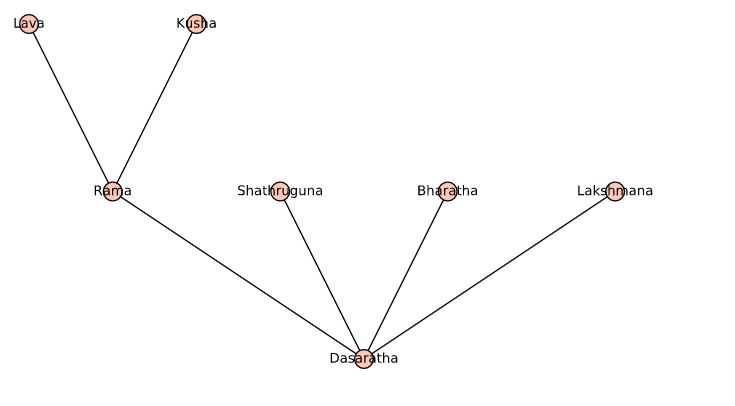
\includegraphics[width=\textwidth]{tree1.JPG}
\caption{A tree drawn with its root at the bottom}\label{rg1}
\end{center}
\end{figure}

\begin{figure}
\begin{center}
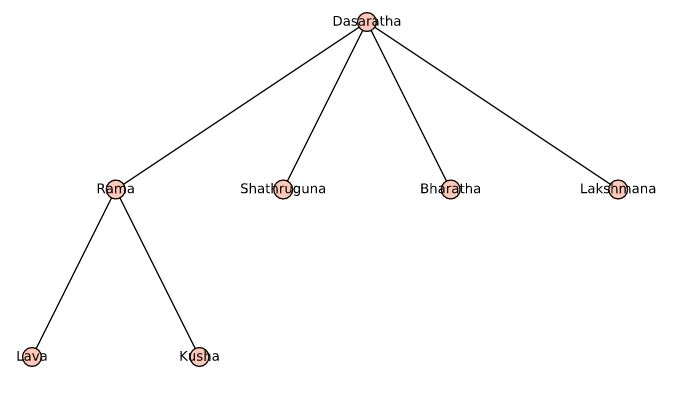
\includegraphics[width=\textwidth]{tree2.JPG}
\caption{The same tree drawn with its root at the top}\label{rg2}
\end{center}
\end{figure}

Rishnak caught up with Ajur and Jura as he had been following them quietly. Rishnak asked Ajur, ``How many edges does a rooted tree with seven vertices have?''

Ajur reasoned that since each vertex other than the root has exactly one parent vertex and there are no other edges, the number of edges will be six.

Rishnak then asked how many edges a rooted tree with 1000 vertices has.

Without blinking, Ajur shot back with his answer. ``Exactly 999.''

Impressed, but not unduly impressed, Rishnak asked how many edges there are in a rooted tree with $n$ vertices.

Nonchalantly, Ajur replied, ``It is $n-1$ by the same argument. I mean each of the $n-1$ vertices has just one edge connected to its parent. For each vertex other than the root vertex, there is a parent vertex and zero or more child vertices.  The descendants\index{descendants} of a vertex are all of its children, grandchildren, great grandchildren, and so on. Analogously, for each vertex, the ancestors of that vertex are its parent, grandparent, great grandparent, and so on.''

Ajur looked up at the trees around him.  ``A vertex with no child vertices is known as a leaf vertex \index{leaf vertex}.''

Rishnak asked Ajur, ``What is the largest number of leaf vertices a tree with six vertices can have?''

Ajur immediately responded that the number is five.  He drew a rooted tree in the dirt [Figure \ref{t1}].

\begin{figure}
\begin{center}
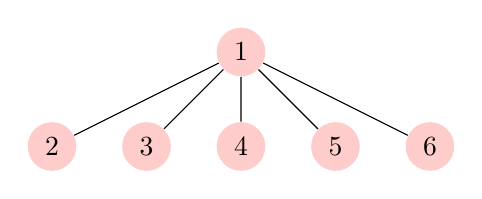
\begin{tikzpicture}
  [scale=.6,auto=left,every node/.style={circle,fill=red!20}]
  \node (n6) at (5,5) {1};
  \node (n4) at (1,3)  {2};
  \node (n5) at (3,3)  {3};
  \node (n1) at (5,3) {4};
  \node (n2) at (7,3)  {5};
  \node (n3) at (9,3)  {6};

  \foreach \from/\to in {n6/n1,n6/n2,n6/n3,n6/n4,n6/n5}
    \draw (\from) -- (\to);

\end{tikzpicture}
\caption{A tree with six vertices and five leaf vertices; the vertex labeled 1 is the root vertex}\label{t1}
\end{center}
\end{figure}

Rishnak asked, ``What is the smallest number of leaf vertices a tree with six vertices can have?''

Ajur knew this answer too. He drew another rooted tree [Figure~\ref{t2}].

\begin{figure}
\begin{center}
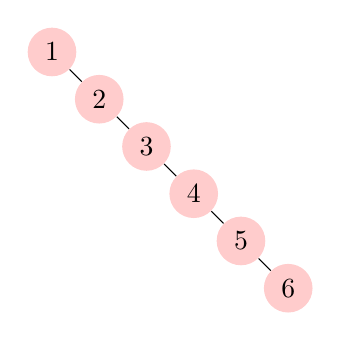
\begin{tikzpicture}
  [scale=.6,auto=left,every node/.style={circle,fill=red!20}]
  \node (n6) at (3,7) {1};
  \node (n4) at (4,6)  {2};
  \node (n5) at (5,5)  {3};
  \node (n1) at (6,4) {4};
  \node (n2) at (7,3)  {5};
  \node (n3) at (8,2)  {6};

  \foreach \from/\to in {n6/n4,n4/n5,n5/n1,n1/n2,n2/n3}
    \draw (\from) -- (\to);

\end{tikzpicture}

\caption{A tree with six vertices and one leaf vertex labeled 6; the vertex labeled 1 is the root vertex}\label{t2}
\end{center}
\end{figure}

Rishnak said, ``We get a lot of lightning and thunderstorms here, especially during the summer months. Lightning affects tall objects in an open area, especially objects that conduct electricity.\footnote{Benjamin Franklin had demonstrated the electrical nature of lightning.} Lightning conductors are usually at the top of buildings and have less resistance than the building. Therefore lightning passes through the conductor.''

In a dazzling light display, Rishnak drew a rooted tree with three vertices [Figure~\ref{t3}]. Rishnak said that each edge has a resistance of 1~ohm, and vertices labeled 2 and 3 are grounded. ``So Ajur, what is the effective resistance of this resistance tree?''

\begin{figure}
\begin{center}

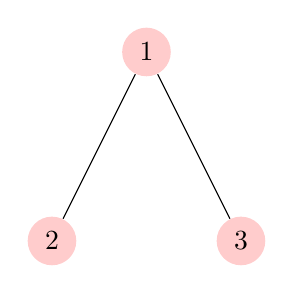
\begin{tikzpicture}
  [scale=.6,auto=left,every node/.style={circle,fill=red!20}]
  \node (n1) at (3,7) {1};
  \node (n2) at (1,3)  {2};
  \node (n3) at (5,3)  {3};


  \foreach \from/\to in {n1/n2,n1/n3}
    \draw (\from) -- (\to);

\end{tikzpicture}

\caption{A resistance tree with three vertices and two leaf vertices as ground}\label{t3}
\end{center}
\end{figure}


Ajur remembered his physics and realized the two resistances were in parallel. He said, ``The effective resistance is $\frac{1}{2}$~ohms.''

Rishnak asked, ``And how do you know that?''

Ajur said, ``Well, intuitively, there are two paths the current can take to reach ground and so the resistance splits evenly between the two paths.''

Rishnak waved his hands through the air and drew another graph that dazzled in front of Ajur's eyes [Figure \ref{t4}].  ``What is the effective resistance for the following rooted tree?''
\begin{figure}
\begin{center}

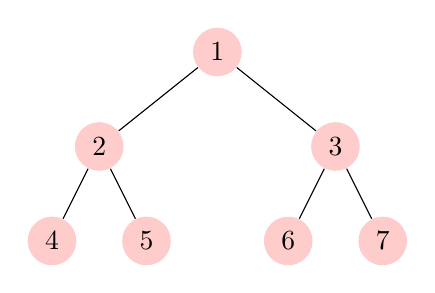
\begin{tikzpicture}
  [scale=.6,auto=left,every node/.style={circle,fill=red!20}]
  \node (n1) at (5.5,7) {1};
  \node (n2) at (3,5)  {2};
  \node (n3) at (8,5)  {3};
  \node (n4) at (2,3) {4};
  \node (n5) at (4,3)  {5};
  \node (n6) at (7,3)  {6};
  \node (n7) at (9,3)  {7};

  \foreach \from/\to in {n1/n2,n1/n3,n2/n4,n2/n5,n3/n6,n3/n7}
    \draw (\from) -- (\to);

\end{tikzpicture}

\caption{A resistance tree with seven vertices and four leaf vertices as ground}\label{t4}
\end{center}
\end{figure}

Ajur said that he had previously computed the effective resistances for the two ``subtrees'' rooted at the vertices labeled 2 and 3 to be $\frac{1}{2}$. From the root, there are two parallel paths with equal resistance of $1+\frac{1}{2}$ (there is a series connection from root vertex 1 to the vertices labeled 2 and 3). Therefore, the effective resistance is half that, or $\frac{3}{4}$~ohms.

Ajur continued, ``There is a pattern here. For the resistance tree with 15 vertices, so adding one more level or increasing the height of this tree, the effective resistance will be $\frac{7}{8}$.''

Rishnak then asked what happens if the tree is of infinite height, a really tall lightning conductor!

Ajur was perplexed. But he reasoned that this could be formulated as a recurrence relation. ``Okay,'' he said, ``let $R$ be the effective resistance of this infinite tree \index{infinite tree}. The root has two children, each of which will have a resistance of $R$ ohms. The root vertex is connected to the child vertex with a resistance of $1$~ohm. Here's the equation.'' He sketched the following equation in the dirt:

$$R= \frac{R+1}{2}$$


\noindent Simplifying this, he concluded that the effective resistance was 1~ohm. ``A tree of infinite height, with its very low resistance, is like a really tall and effective lightning conductor.''\footnote{Ajur was right, but because of the large number of joints, this solution may not be a practical one!}

\newpage
Rishnak stated that there was another way of getting the same result. Smiling, he said, ``From an earlier example, you can generalize the resistance to be~$\frac{2^h-1}{2^h}$, where $h$ is the height of the rooted tree. The height here is the longest of path lengths from the root vertex to all of its leaf vertices. What can that equation be simplified to?''

Ajur thought for a moment, then said, ``It can be further simplified to~$1-\frac{1}{2^h}$.''

Rishnak smiled again. ``And as~$h$ goes to infinity, the~$\frac{1}{2^h}$ term goes to zero and hence the resistance is simply~$1$.''

Ajur stood in awe. He learned the important lesson that there are often multiple ways of finding a solution, and each approach may provide a new insight.

Ajur asked Rishnak, ``Can you construct a tree with infinite height (so with an edge resistance of 1~ohm) so that the effective resistance is~$\frac{1}{2}$, $\frac{1}{3}$, $\frac{1}{4}$, or more generally any fraction less than or equal to 1?''

Rishnak frowned. ``I'm the one asking the questions.''\footnote{Of course Rishnak knew the answer and suggests that you answer this by thinking of every vertex with more than two child vertices.}

Rishnak cleared his throat and continued. ``A tree is like a rooted tree but with no root vertex. A tree can be drawn in any manner. The degree of a vertex is the number of edges incident on that vertex. The leaf or pendant vertex has a degree of~1. So in this tree [Figure~\ref{t2}], both vertices labeled~1 and 6 are leaf or pendant vertices, while all other vertices have degree~2.''

Rishnak told Ajur that one important property of a tree is that there are no cycles in it. Ajur could easily understand this from a genealogy perspective---a person cannot be an ancestor as well as a descendant of himself or herself.
Ajur thought further and said, ``There is only one path between any two vertices in a tree.''

Of course Ajur assumed that the edges were undirected, which Rishnak knew. Rishnak asked, ``How did you infer that there is a unique path between two vertices in a tree?''

Ajur promptly replied that if there are two paths between any two vertices, there will be a cycle, which cannot exist in a tree. Since there is a unique path between two vertices, one can compute the distance between two vertices as the number of edges in that path.

Ajur provided clarifications with some examples. As one example, in this first tree that I drew [Figure~\ref{t1}], the distance between the vertex labeled~1 and any other vertex is~1. And the distance between the vertex labeled~2 and the vertex labeled~6 is~2.''

Rishnak nodded as Ajur continued. ``In this other tree [Figure~\ref{t2}], the distance between the vertex labeled~1 and the vertex labeled~6 is~5, while the distance between the vertex labeled~2 and the vertex labeled~5 is~3, and the distance between the vertex labeled---''

``Okay, I got it,'' boomed Rishnak.
%(Dad: you could also add the fact that every finite tree has a center of mass! it's in this vein, and not especially well known (Boris hadn't realized it!))

\subsection*{Question for the second day}
Rishnak stood tall. ``Ajur, here is the question for the second night. Can you construct an infinite tree with an effective resistance of $\frac{3}{5}$?''

\textit{Before you turn the page, try to come up with an answer of your own!}

\newpage
\subsection*{Answer for the second day}
Ajur repeated the question to himself, wondering how to solve it. ``An infinite tree with an effective resistance of~$\frac{3}{5}$?''

Rishnak said, ``Well?''

Ajur said, ``A way to think about this is to consider an infinite tree in which each vertex has six children and each edge is of resistance 3~ohms. We can add a series of three 1~ohm edges to get to 3~ohms.''

Rishnak said, ``Are you sure that will work?''

Ajur said, ``Yes, with this tree, we will get this recurrence equation.''  He quickly sketched out the recurrence in the dirt:

$$R=\frac{R+3}{6}$$

\noindent Here, each child vertex will have a resistance of $R$~ohms (by symmetry, as they look like the original tree). Simplifying this, we get~$\frac{5R}{6}=\frac{3}{6}$, which if we solve for~$R$ gets us to a resistance of~$R=\frac{3}{5}$~ohms.''

Rishnak was very pleased. Jura barked and they called it a night.